\documentclass[KITtoc]{beamer}
\mode<presentation>
{
  \usetheme[english,titlepage0]{KIT}
  %\setbeamercovered{transparent}
  %\setbeamertemplate{enumerate items}[circle]
}

\TitleImage[width=\titleimagewd]{img/KIT-Titel7}

\usepackage{etex}
\usepackage[utf8]{inputenc}
\usepackage[T1]{fontenc}
\usepackage{array}
\usepackage{multicol}
\usepackage{ragged2e}
\usepackage{bbm}
\usepackage{algorithmic}
\usepackage{marvosym}
\usepackage{listings}

\usepackage{tikz,pgfplots}
\usetikzlibrary{calc,positioning,arrows,shapes}
\usetikzlibrary{decorations.pathreplacing}

\makeatletter
\def\slot[#1,#2](#3);{{
	\draw  (#3,0) rectangle (#3+0.5,0.5) node[midway] (#2) {#1};
}}
\makeatother

\RequirePackage{xcolor}

\newcommand<>{\galert}[1]{{\color#2{KITgreen}#1}}
\newcommand<>{\balert}[1]{{\color#2{KITblue}#1}}
\newcommand<>{\ralert}[1]{{\color#2{KITred}#1}}

\title[\textbf{Candy Kingdom meets HordeSAT}]{\textbf{CandyHorde: Candy Kingdom meets HordeSAT}}
\subtitle{Markus Iser}
\author[Markus Iser]{Markus Iser}
\institute[Karlsruhe Institute of Technology (KIT)]{KARLSRUHE INSTITUTE OF TECHNOLOGY (KIT)}

\begin{document}

\begin{frame}
\maketitle
\end{frame}

\begin{frame}{Candy}

\url{https://github.com/Udopia/candy-kingdom}

\begin{block}{Candy}
\begin{itemize}
\item Fork of Glucose (MiniSAT)
\item Modern C++
\item Modularity: Separation of Concerns
\item Simplicity: Use of Standard Library
\end{itemize}
\end{block}

\begin{block}{New Sub-Systems}
\begin{itemize}
\item Structure Analysis and Random Simulation (Gates, Tseitin)
\item Structure-based Branching (RSIL)
\item Structure-based Abstraction (RSAR)
\item Structure-based Model Minimization
\end{itemize}
\end{block}

\end{frame}

\begin{frame}{Candy Systems}

\begin{block}{Candy Systems}
\begin{itemize}
\item Clause Database (Clause, Clause Allocation)
\item Current Assignment (Trail)
\item Propagation System (Watchers)
\item Clause Learning System (Conflict Analysis, 1-UIP Learning)
\item Branching System (VSIDS, LRB, RSIL)
\end{itemize}
\end{block}

\end{frame}

\begin{frame}[fragile]{Candy Static Polymorphism}
\begin{block}{Candy Initialization}
\small
\begin{lstlisting}
TDb*     clauses    = new TDb    ();
TTrail*  assignment = new TTrail ();

TProp*   propagate  = new TProp  (db, assignment);
TLearn*  learning   = new TLearn (db, assignment);
TBranch* branching  = new TBranch(db, assignment);

Candy* solver = 
  new Solver<TDb, TTrail, TProp, TLearn, TBranch> (
    clauses, assignment, propagate, learning, branching
  );
\end{lstlisting}

\end{block}
\begin{itemize}
\item TBranch: VSIDS, LRB, RSIL, \dots
\item TTrail and TPropagate now have ``ThreadSafe'' Variants
\end{itemize}
\end{frame}

\begin{frame}{Recent Candy Development}
\begin{block}{``Halloween'' Version vs Recent Version ``Cain''}
\begin{columns}
\column{.6\linewidth}
\includegraphics[width=\linewidth, trim=30 0 50 0, clip]{plots/halloween-vs-cain.eps}
\column{.4\linewidth}
\small
\textbf{Halloween:}\\
Solved: 129/400\\
PAR-2: 2909362\\~\\
\textbf{Cain:}\\
Solved: 146/400\\
PAR-2: 2772256\\
\end{columns}
\end{block}
\end{frame}

\begin{frame}{Compared to ``Mother'' Glucose}
\begin{block}{Still Worse Performance}
\begin{columns}
\column{.6\linewidth}
\includegraphics[width=\linewidth, trim=30 0 50 0, clip]{plots/glucose-vs-cain.eps}
\column{.4\linewidth}
\small
\textbf{Glucose:}\\
Solved: 171/400\\
PAR-2: 2502445\\~\\
\textbf{Cain:}\\
Solved: 146/400\\
PAR-2: 2772256\\
\end{columns}
\end{block}
\end{frame}

\begin{frame}{HordeSAT}
https://github.com/biotomas/hordesat
\begin{block}{HordeSAT Parallel Interface}
\begin{itemize}
\item Highly configurable parallel solver implementation
\item Abstracts away details of single solver implemenation
\item Can run portfolio of solvers
\item Implementation of Horde interface: Lingeling, Minisat and now \dots
\item \dots \textbf{Candy!}
\end{itemize}
\end{block}
\end{frame}

\begin{frame}{Candy Horde}
\includegraphics[width=\linewidth]{img/candy-horde.png}
\end{frame}

\begin{frame}{First Results}
\begin{block}{One vs. Two Instaces of Candy Version ``Cain''}
\begin{columns}
\column{.6\linewidth}
\includegraphics[width=\linewidth, trim=30 0 50 0, clip]{plots/cain-one-vs-two.eps}
\column{.4\linewidth}
\small
\textbf{Single Cain (VSIDS):}\\
Solved: 146/400\\
PAR-2: 2772256\\~\\
\textbf{Parallel Cain (VSIDS \& LRB):}\\
Solved: 156/400\\
PAR-2: 2559229\\~\\
no clause-sharing or additional diversification so far
\end{columns}
\end{block}
\end{frame}

\begin{frame}{Solving the Memory Problem}
\begin{block}{Sharing of Clause Database}
\begin{itemize}
\item Modularity of Candy makes it easy to share one Clause Database across solver instances
\item However, propagate and clause-learning sub-systems utilize order of literals in clauses
\item New implementations of propagate and clause-learning sub-systems must operate without changing or exploiting literal-order
\end{itemize}
\end{block}
\end{frame}

\begin{frame}{Literal Order}
\begin{block}{First Two Literals in Clause are Watched}
\begin{itemize}
\item The first literal is the the asserted (true) literal
\item The second literal is the propagation trigger / the other watched literal
\item Advantage: Watchers are independent (one watcher for each of the two literals)
\end{itemize}
\end{block}
\end{frame}

\begin{frame}{Refactoring the Solver}
\begin{block}{Step-by-step}
\begin{itemize}
\item Make all non-const methods in clause ``private''
\item Mark classes that access these methods as ``friends''
\item Reduce the number of friends to clauses (until only propagate and clause-analysis remain)
\item Write new propagate and clause-analysis that are not friends of clause
\end{itemize}
\end{block}
\end{frame}

\begin{frame}{Building a literal-order invariant Conflict Analysis}
Advantage: Can be tested indepentent of Propagator
\begin{block}{Step-by-step}
\begin{itemize}
\item Make all non-const methods in clause ``private''
\item Mark classes that access these methods as ``friends''
\item Reduce the number of friends to clauses (until only propagate and clause-analysis remain)
\item Write new propagate and clause-analysis that are not friends of clause
\end{itemize}
\end{block}
\end{frame}


\begin{frame}[fragile]{Conflict Analysis becomes Easier}
\begin{block}{Legacy Clause Analysis}
\small
\begin{lstlisting}
if (confl->size() == 2 && trail.value(confl[0]) == l_False) {
  confl->swap(0, 1);
}
auto it = isbegin() ? confl->begin() : confl->begin() + 1;
for (; it != confl->end(); it++) {
  Var v = var(*it);
  if (!stamp[v] && trail.level(v) != 0) { ... }
}
\end{lstlisting}
\end{block}

\begin{block}{New Clause Analysis}
\small
\begin{lstlisting}
for (Lit lit : *confl) {
  Var v = var(lit);
  if (lit != aslit && !stamp[v] && trail.level(v) != 0) { ... }
}
\end{lstlisting}
\end{block}
\end{frame}

\begin{frame}{First Results}
\begin{block}{Candy Version ``Cain'' with Classic vs. New Conflict Analysis}
\begin{columns}
\column{.6\linewidth}
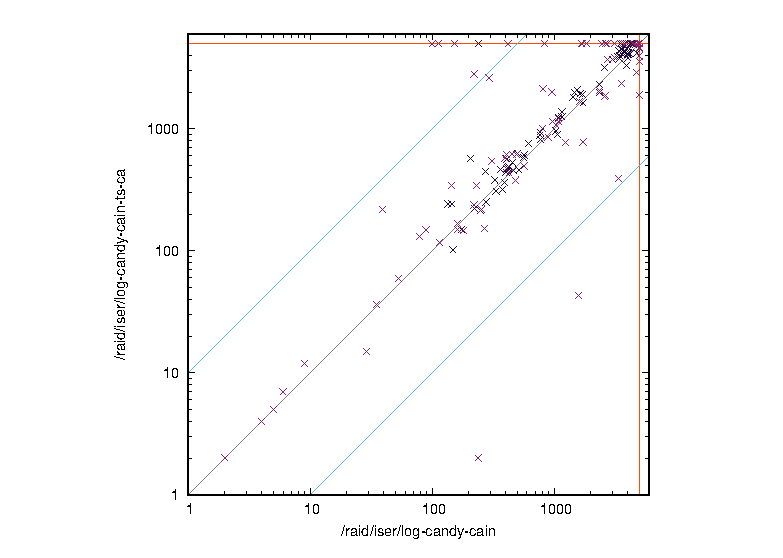
\includegraphics[width=\linewidth, trim=30 0 50 0, clip]{plots/cain-ca-vs-sca.eps}
\column{.4\linewidth}
\small
\textbf{Classical Cain:}\\
Solved: 146/400\\
PAR-2: 2772256\\~\\
\textbf{New Cain:}\\
Solved: 128/400\\
PAR-2: 2923940\\
\end{columns}
\end{block}
\end{frame}

\end{document}
